\documentclass[a4paper, top=10mm]{article}
%for writing from the top
\usepackage{fullpage}
%for math
\usepackage{amsmath}
\usepackage{mathrsfs}
\usepackage{amsthm}
\usepackage{amsfonts}
%for images
\usepackage{graphicx}
%for color
\usepackage{xcolor}
%for title
\title{\textbf{\huge{Terrace}}}
\author{Enigma n\textsuperscript{o}7}
\date{2\textsuperscript{nd} December 2022}

\newtheorem*{hint}{Hint}

\addtolength{\voffset}{-2cm}
\addtolength{\textheight}{5cm}


\begin{document}
	\maketitle
	
	A gardener is leaving a square of grass in the middle of his terrace.
	He is wondering how much grass he should buy.
	He would need the area of the square he left empty.
	The terrace is square of side 10m.
	The middle square is outlined by ropes going from the terrace corner to the middle of the opposing side as shown below:
	
	\vspace{0.5cm}
	
	\begin{center}
		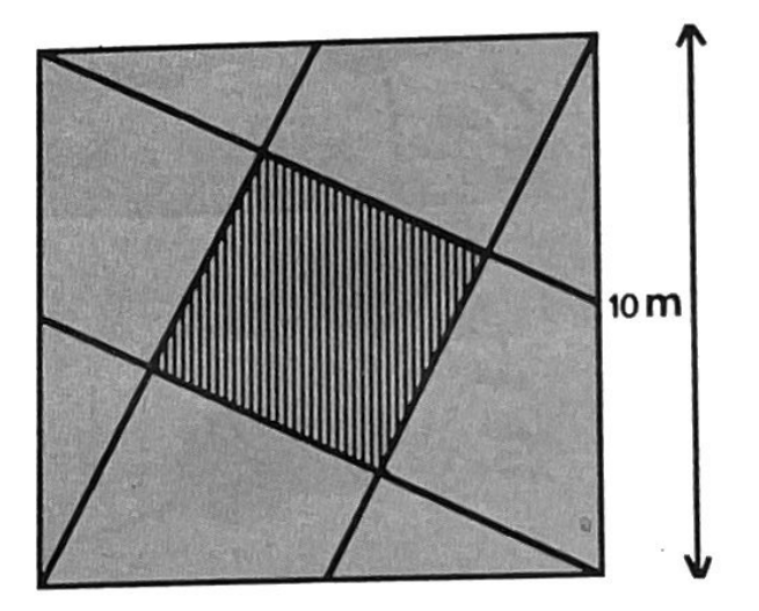
\includegraphics[height=200pt]{07pavement.png}\\
		Terrace schema.
	\end{center}
	
	\vspace{3cm}
	
	\textbf{Find the area of the middle square in squared meter (rounded to the closes integer if needed).}
	
\end{document}